\section{Proof with and without probability}\label{without}

Here we locate the approach presented in \citet{verheijProofProbabilities2017} within the research field and the related literature.

In \cite{verheijProofProbabilities2017}, argumentation is applied in the context of forensic science. There, the training data consist of scenarios of abstract propositions. Without changing the essence of the approach too much, we can reinterpret this framing and conceive of the training data as a boolean representation.

Verheij defines three kinds of arguments, of which \textit{(presumptively) valid arguments} are most interesting. They are probabilistically valid (or alternatively, valid based on the preference relation between cases). In this, they resemble association rules. 

The primary target audience in \cite{verheijProofProbabilities2017} is rather forensic science than machine learning. The conceived user story for the model may be a group of criminal investigators who hypothesize about what happened during a crime (see the case study in section 5 of that paper). In the course of their investigations, they draw up case models at their board, and revise them as new evidence arrives. 

The more general target of the approach that is presented in \cite{verheijProofProbabilities2017}, however, is its application to machine learning: \say{[I]t is not a big step to view the cases in a case model as the data that can be used for learninglike in data systems—and the rules that are valid in it as the knowledge structure of knowledge systems.} \citep[p.~66]{verheijArgumentsGoodArtificial2018}

\cite{verheijProofProbabilities2017} has been compared with another hybrid qualitative-quantitative reasoning model based on Bayesian networks in \citet{vanleeuwenComparisonTwoHybrid2019}. The model of \cite{verheijProofProbabilities2017} has been tested in the paper itself for investigating the murder in the Alfred Hitchcock movie \textit{To catch a thief}, with hand-made examples. Subsequently, it has been applied to a real criminal case, the \textit{Simonshaven case} \cite{verheijAnalyzingSimonshavenCase2020}. The latter analysis was undertaken for a conference\footnote{\url{https://onlinelibrary.wiley.com/toc/17568765/2020/12/4}}, as part of which multiple authors have applied their formal models to investigating the Simonshaven case. The competing approaches presented at the conference are argumentation-based analysis, Bayesian networks, Bayesian thinking, scenarios, and a hybrid approach using stories and arguments. \citet{verheijAnalyzingSimonshavenCase2020} has been reviewed in \cite{zenkerStoriesviaArgumentsScenarios2020}.

\begin{figure}[htb]
        \centering
        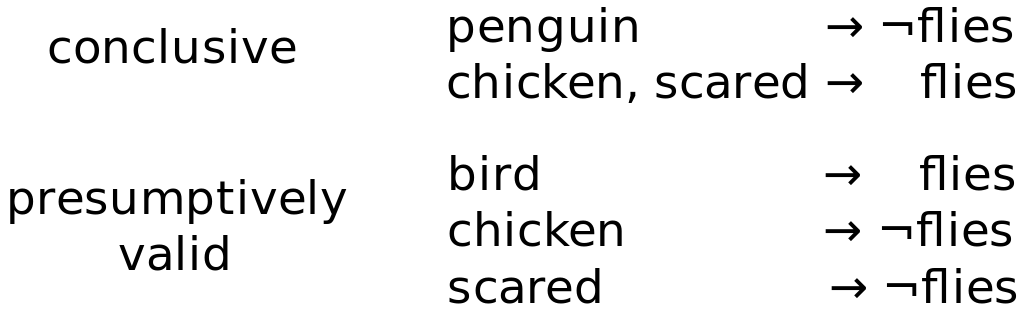
\includegraphics[width=0.5\textwidth]{images/arguments.png}
        \caption{Some fictitious conclusive and (presumptively) valid arguments for the argumentation approach of \cite{verheijProofProbabilities2017}.}
        \label{fig:arguments}
\end{figure}


\section{Reasoning with rules and arguments}

The formal study of argumentation is only relatively recent. Historically, classical logic has often been used instead. Classical logic is monotonic, meaning that additional information cannot revise conclusions that would have been made otherwise. The computational implementation and application of classical logic is recently studied especially using \textit{miniKanren}\footnote{\url{http://minikanren.org/\#implementations}}, a logic programming language embedded into other programming languages.

Because the satisfiability of sentences (and, hence, also entailment between them) are neither generally decidable nor efficiently computable for classical logic, logic has often been restricted to \textit{Horn clauses} in artificial intelligence, which fare better in these respects \citep[ch.~7.5.3]{russellArtificialIntelligenceModern2010}. Horn clauses are disjunctions of literals (that is, variables or predicate expressions representing atomic facts), where exactly one literal is positive. More intuitively, they are a rule from a conjunction of positive literals to another positive literal. The \textit{Prolog} family of programming languages enables efficient reasoning with Horn clauses of predicates. \footnote{For example, \url{https://www.swi-prolog.org/}, \url{http://www.gprolog.org/}, \url{https://ciao-lang.org/}} By means of recursive predicates, it also allows for programming. Prolog has been extended to allow for negations by a mechanism known as \textit{negation as failure}. The ProbLog programming language extends Prolog with probability theory.\footnote{\url{https://dtai.cs.kuleuven.be/problog/}} 

Argumentation has been formalized on an abstract level by \citet{dungAcceptabilityArgumentsIts1995}: An argument is the connection between some premises (the \textit{support} of the argument) and a conclusion. Arguments can attack each other. An argument is defeated either if is \textit{rebutted} by another argument, or if one of its premises is rebutted by another argument, in which case the argument itself is \textit{undercut}. Abstract argumentation has been implemented in \textit{ASPIC+} \citep{modgilASPICFrameworkStructured2014}. 

Argumentation in the context of logic has been formalized, for example, by \citet{roosResolvingConflictsArguments2000}. A \textit{defeasible theor}y consists of \textit{facts}, \textit{strict rules}, and \textit{defeasible rules}. The defeasible rules are partially ordered by a \textit{preference relation}, such that in the case of conflicting rules, the conflict can be resolved by ignoring the less preferred rule. 

The preference relation can be derived using the criterion of \textit{specificity} between rules \citep[def.~4]{roosResolvingConflictsArguments2000}. An argument is more specific than a second argument if from the premises of the argument an argument can be made to the premises of the second argument. An argument is strictly more specific than a second argument if it is more sepcific than the second argument and the second is not more specific than the first argument. When using specificity to derive the preference relation of a defeasible theory, more specific rules will be preferred to less specific rules. 

Reasoner implementations for defeasible argumentation (in various flavours) include \textit{SPINdle}\footnote{\url{https://github.com/NICTA/SPINdle}} in Java, \textit{DePYsible}\footnote{\url{https://github.com/stefano-bragaglia/DePYsible}} in Python, \textit{Oscar}\footnote{\url{https://web.archive.org/web/20170806211112/http://johnpollock.us/ftp/OSCAR-web-page/oscar.html}} in Common Lisp. A variety of further argumentation libraries is maintained by the \textit{TweetyProject}\footnote{\url{http://tweetyproject.org/lib/index.html}}. Recently, a semantic tableau reasoner has been proposed \citep{roosSemanticTableauMethod2020} and implemented \citep{barbarafutymaExplainableAIArguments2021}; the advantage of the semantic tableau proof method is that it is comparatively easy for humans to understand (as compared to resolution or natural deduction).

\section{Learning arguments}

In order to participate in argumentation, it is necessary to know a set of rules. Then, facts and rules can be combined to arguments, and the conclusions from the arguments can be used to construct more arguments.

Many different approaches in data mining and machine learning are concerned with the learning of rules. Here, we give a broad overview over techniques for learning rules. We do not only cover rules in the narrower sense as used within defeasible argumentation, but in the broader sense as used within explainable artificial intelligence. This is because many insights about efficient mining techniques, as well as about the limitations of rule learning, can be transferred from this wider set of approaches to the approach here investigated. 

\citet{deraedtLogicalRelationalLearning2008} introduces a hierarchy of machine learning representations, from simple to complicated:

\begin{enumerate}
\item \textit{Boolean} (or \textit{binary}) representation, that is, each data point is a set of propositions.
\item \textit{Attribute-value} representation, typical for most standard machine learning algorithms.
\item \textit{Multi-instance} representation, where multiple rows can belong to one data point.
\item \textit{Relational} representation, where multiple interconnected tables are used.
\item \textit{Logic program} representation, where functors and structured terms turn the data into a turing-complete programming language such as Prolog. 
\end{enumerate}

This hierarchy will be useful in seeing the different (original) application areas of the presented machine learning techniques. It should also be noted that it is systematically possible to transfer a technique to work on higher-level or lower-level representations. \citet[ch.~6]{deraedtLogicalRelationalLearning2008} have demonstrated this by upgrading a propositional rule learner, an attribute-value decision tree learner, and a propositional frequent item set miner, all to work on relational data.

The learning of rules can be considered either \textit{unsupervised learning}, when the rules are considered the product; or it can be considered \textit{supervised learning}, when the rules are considered to be a tool for conducting further analysis, as in \textit{rule-based classification}. In the latter case, the task \textit{can} be restricted to learning only rules for directly predicting the relevant attributes.

We broadly cluster the existing approaches into the following categories. The boundaries between these categories are very fluid.

\begin{enumerate}
    \item \textit{Argumentation and (defeasible) logic rules.} This is most close to the approach investigated in the project.
    \item \textit{Classification rules.} These are used for rule-based classification, and do not aim to be understandable, but merely to be a tool for classification. 
    \item \textit{Probabilistic and causal models.} They allow for quantitative reasoning.
\end{enumerate}

\subsection{Argumentation, logic, and association in machine learning}

\citet{kakasAbductionArgumentationExplainable2020} differentiate between multiple use cases of argumentation in machine learning: Inputs extended with arguments (most prominently, \textit{argument-based machine learning, ABML}); inputs interpreted as arguments; hypotheses interpreted as arguments; and hypotheses expressed in argumentation. The last use case, where argumentation is the \textit{target language} for learning \citep[p.~17]{kakasAbductionArgumentationExplainable2020}, is the one that is relevant for this project. \citet{kakasAbductionArgumentationExplainable2020} further distinguish two paradigms within this use case: 

\begin{itemize}
    \item In the first paradigm, arguments are monolithic rules that directly map input facts to output facts. This paradigm comprises decision lists, exception lists, exceptions in inductive logic programming, and random forest methods.
    \item In the second paradigm, arguments may consist of multiple chained smaller rules that are chained together, with intermediate concepts connecting the rules. Examples are the \textit{never-ending rule discovery (NERD)} algorithm, \textit{machine coaching}, and \textit{simultaneous learning and prediction (SLAP)}. 
\end{itemize}

\subsubsection{Learning defeasible rules}\label{sec:defeasible-rules}

\begin{figure}[htb]
        \centering
        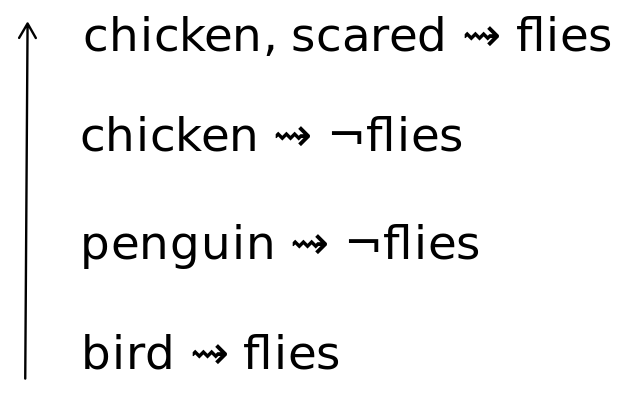
\includegraphics[width=0.3\textwidth]{images/defeasible-theory.png}
        \caption{A fictitious defeasible theory from aviational zoology. The arrow represents the preference relation. Note that the preference relation is total here, but it can also be partial.}
        \label{fig:defeasible-rules}
\end{figure}

Two algorithms are explicitly concerned with learning defeasible rules. The first, \textit{DefGen} uses as a basis the results of an association rule miner (see \autoref{sec:association-rules}), and then applies relevance criteria to the learned rules \cite{governatoriApplicationAssociationRules2001}.

Learning from the drawbacks of \textit{DefGen}, \textit{HeRo} has been developed to mine defeasible rules independently of an association rule miner \cite{johnstonAlgorithmInductionDefeasible2003}. \textit{HeRo} takes inspiration from decision tree learners, with its incremental algorithm that uses \textit{information gain} as a core criterion (see \autoref{sec:decision-trees}). The structure of the algorithm resembles decision list algorithms and covering rule algorithms (see \autoref{sec:decision-lists}).

\subsubsection{Learning logical rules and logic programs}

\begin{figure}[htb]
        \centering
        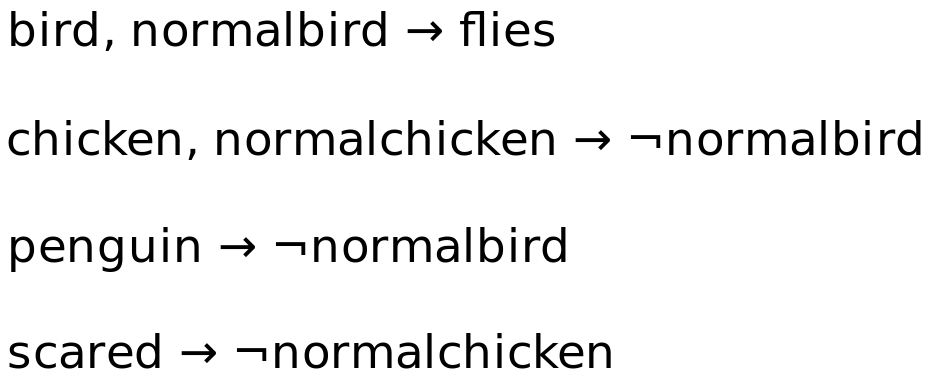
\includegraphics[width=0.4\textwidth]{images/monotonic-theory.png}
        \caption{A fictitious set of monotonic rules. Here, a normality predicate is used in order to capture what would otherwise be captured by using defeasible rules. The approach of using normality predicates is found, among other places, in some examples in de Raedt 2008. It has been adapted here to a normality proposition for each originally defeasible rule.}
        \label{fig:relational}
\end{figure}

Relational learning is similar to the learning of defeasible rules, but it typically produces monotonic rules (that is, in this context, rules which are always valid regardless of any other rules). Like association rule learning, relational learning is concerned with the discovery of patterns in the training data \citep{deraedtLogicalRelationalLearning2008}. The difference is that relational learning works on relational representations, and, in part, on logic program representations. The technique is generally applied to predicate logic. It can be downgraded to propositional logic, which would make it applicable to the task of this project. A particularly interesting discovery in relational learning is that it is possible for algorithms to create new predicates that are not present in the training data \citep[p.~797f.]{russellArtificialIntelligenceModern2010}. Potentially, such predicate invention could lead to smaller, more local rules. The invention of new predicates is also considered a crucial skill for the induction of new scientific theories \citep[p.~797f.]{russellArtificialIntelligenceModern2010}.

Particular research effort within relational learning is going into \textit{inductive logic programming}, where Prolog programs are learned from examples. Such methods can successfully learn programs like fizz-buzz from very few examples. A notable example of an inductive logic program learner is the \textit{first-order inductive learner} (\textit{FOIL}; \citet{quinlanLearningLogicalDefinitions1990}), which can be viewed as an extension of covering rule algorithms (see \autoref{sec:decision-lists}) to first-order logic \citep[p.~362f.]{hanDataMiningConcepts2011}. Further algorithms include the \textit{model inference system (MIS)}, and \textit{Progol}, which improves upon FOIL and MIS. 

Notably, there are inductive logic programming algorithms for learning nonmonotonic rules, for example, \textit{XHAIL}\footnote{\url{https://github.com/stefano-bragaglia/XHAIL}}, and \textit{top-directed abdutcive learning} (\textit{TAL}; see \citet{corapiInductiveLogicProgramming2010}). \citet{dimopoulosLearningNonmonotonicLogic1995} present a theoretical framework for nonmonotonic inductive logic learning.

\cite{kakasAbductionArgumentationExplainable2020} stress the importance of combining inductive with abductive approaches within relational learning. Such algorithms use an inductive-abductive cycle. That is, they induce rules, then create new eamples based on these rules, which in turn make it possible to induce new rules.

\subsubsection{Learning association rules and exception rules}\label{sec:association-rules}

\begin{figure}[htb]
        \centering
        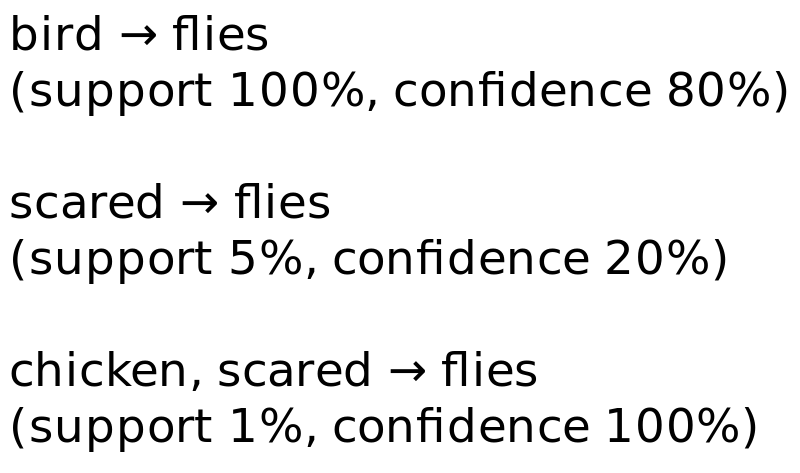
\includegraphics[width=0.4\textwidth]{images/association-rules.png}
        \caption{A fictitious set of association rules with important measures, from a fictitious bird database.}
        \label{fig:association-rules}
\end{figure}

Association rule mining is a classical data mining task. It works on boolean representations. Its paradigmatic application is shopping basket analysis, where customers of an online shop receive recommendations based on what other customers with a similar basket have tended to buy in the past. Association rule mining is efficiently possible with the \textit{Apriori algorithm} \citep{agrawalFastAlgorithmsMining1994}. (And subsequently to the Apriori algorithm, many versions with additional optimizations have been developed.) The algorithm makes use of two observations about the search space: 

\begin{itemize}
    \item First, association rules with $n$ premises can be found by mining frequent sets of $n + 1$ items, then for each item in the set creating a rule with that item as a consequence of the other items. So, for rules with a single premise, we could mine frequent sets with 2 members, and when we find, for example, the set ${a, b}$ with frequency $p$, we can create one rule $a \rightarrow b$, and one rule $b \rightarrow a$. (The \textit{confidence} measure will need to be calculated again for all of the resulting rules; but not the \textit{support} measure, which is handy; see \citet[p.~350]{tanIntroductionDataMining2014}.
    
    \item Second, we do not need to search for frequent sets, when a subset of them is already below a threshold such that we consider it infrequent. This is due to the Apriori principle: \say{If an itemset is frequent, then all of its subsets must also be frequent.} \citep[p.~333]{tanIntroductionDataMining2014} 
    
    \autoref{fig:pruning} shows that this technique allows for pruning of the search space with dramatic effects. (\citet{deraedtLogicalRelationalLearning2008} transfer this pruning technique to relational learning in general.)
\end{itemize}

\begin{figure}[htb]
        \centering
        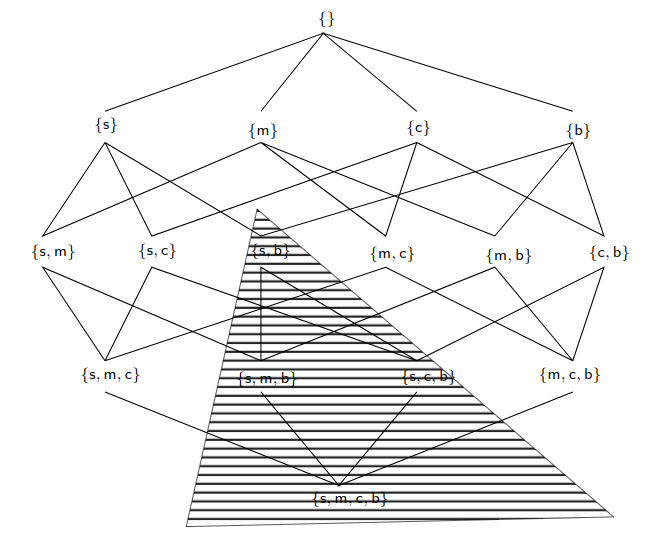
\includegraphics[width=0.6\textwidth]{images/pruning.png}
        \caption{\textit{Pruning specializations.} From \citet[p.~52]{deraedtLogicalRelationalLearning2008}. All $2^n$ subsets of $\{s, m, c, b\}$ are systematically searched, starting from the most general set at the top. Knowing that the set $\{s, b\}$ is infrequent allows us to prune all its specializations, which is a lot. }
        \label{fig:pruning}
\end{figure}

Association rules typically come with two main metrics: The \textit{support} (or \textit{coverage}) indicates the frequency of the premises of the rule. The \textit{confidence} (or \textit{accuracy}) indicates for which share of these data the conclusion of the rule does apply. Additional measures are used to establish whether a rule is interesting and should be kept: The \textit{lift} is the most important of these measures. It measures how much more likely the premises and conclusion are to occur together, in comparison to the case that the premises and the conclusion were conditionally independent. 

$$\text{lift}(A\rightarrow B)=\frac{\text{support}(A \land B)}{\text{support}(A)\cdot\text{support}(B)}$$

\citet[ch.~6]{tanIntroductionDataMining2014} describe the process of mining frequent item sets and association rules with various optimizations in detail. They also give a broader overview over evaluation measures for association rules. \cite[ch.~7]{tanIntroductionDataMining2014} considers advanced techniques, for dealing with categorical and continuous data. 

The topic of \textit{exception rules} has been investigated within the context of association rule mining (see, for example, \citet{taniarExceptionRulesAssociation2008}). Exception rules are typically ordered in a hierarchy of rules, exceptions, exceptions to the exceptions, and so forth. This hierarchical representation is similar to a representation using a preference relation on rules, where a rule receives a lower preference than the exceptions to it \citep[p.~81f.]{wittenDataMiningPractical2017}. As far as we see, it seems that the research fields of \textit{exception rules within association rule mining} and of \textit{defeasible rules within the context of logic and argumentation} are not much mutually aware of each other.

\subsection{Learning classification rules}

Classification rules aim exclusively at supervised learning, where they are used as a mere tool; the rules are optimized for accuracy rather than for explainability. (Within the domain of supervised learning, they are still more explainable than most alternative approaches.) Classification rules are interesting mainly because of the pruning techniques developed for them, and for two special cases of them, regression trees and decision lists. These three points may be transferable to the problems faced in this project. 

\subsubsection{Decision trees}\label{sec:decision-trees}

\begin{figure}[htb]
        \centering
        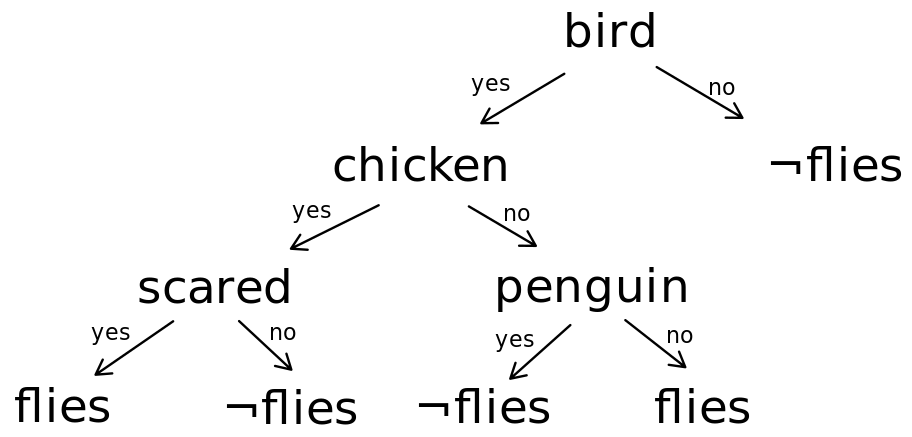
\includegraphics[width=0.5\textwidth]{images/decision-tree.png}
        \caption{A fictitious decision tree.}
        \label{fig:decision-tree}
\end{figure}

Decision trees are one of the most popular methods in machine learning, and --within the domain of supervised learning-- especially suited for explainability, since they can easily be executed by a human \cite[ch.~18.3]{russellArtificialIntelligenceModern2010}. They work on attribute-value representations with binary as well as (by simple extensions) with categorical and continuous data.

However, \citet{breidenbachTextCode2021} notes that decision trees go the wrong way for explainability: Decision trees start with the assumptions and end with the conclusions. The same conclusion may be derived at the end of many different branches. Human reasoning, in contrast, starts with the conclusion and ends with all the different nested assumptions (that is, it uses argumentation). 

Decision trees are mined by iteratively applying the criterion of information gain. The criterion of information gain tells which attribute should be used next (see \citet[ch.~18.3]{russellArtificialIntelligenceModern2010}; \citet[ch.~4.3]{wittenDataMiningPractical2017}). Decision trees can be pruned, which improves accuracy, because it avoids overfitting, and in turn also makes the rules simpler. 

A decision tree can be regarded as a set of \textit{classification rules} that can be used together (\citet[ch.~3.4]{wittenDataMiningPractical2017}; \citet[p.~358]{hanDataMiningConcepts2011}). Each classification rule involves all the criteria along a branch from the root node to the leaf node with the decision. This has the disadvantage that the rules may be very long, and the advantages that each rule is always very accurate, and that there are no conflicts between the rules.

\subsubsection{Regression trees}

\begin{figure}[htb]
        \centering
        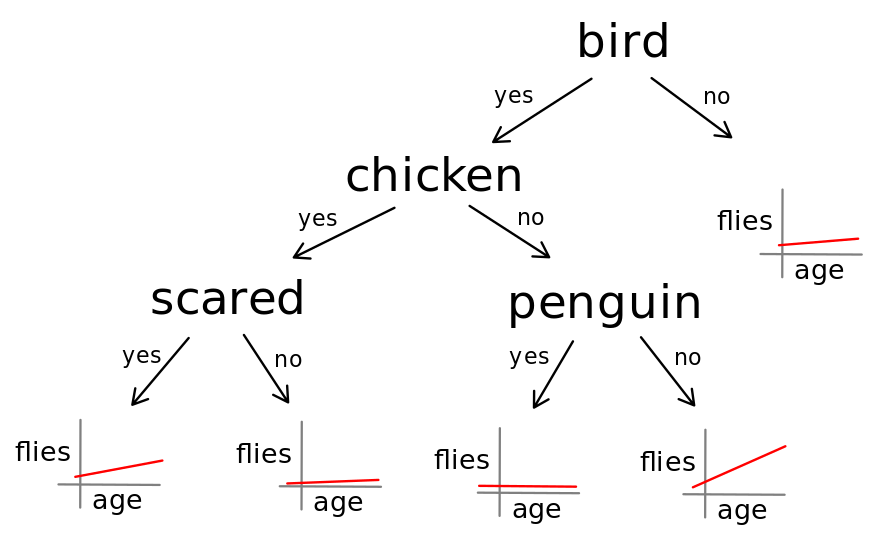
\includegraphics[width=0.5\textwidth]{images/regression-tree.png}
        \caption{A fictitious regression tree. Unlike in this example, where the regression models in the leafs node are about an additional attribute, the regression models may as well be about continuous attributes that are already involved (in discretized form) in the decision structure of the tree.}
        \label{fig:regression-list}
\end{figure}

Regression trees extend decision trees to work on continuous data without discretizing the predicted attribute \citep[p.~72ff.]{wittenDataMiningPractical2017}).

\subsubsection{Decision lists}\label{sec:decision-lists}

\begin{figure}[htb]
        \centering
        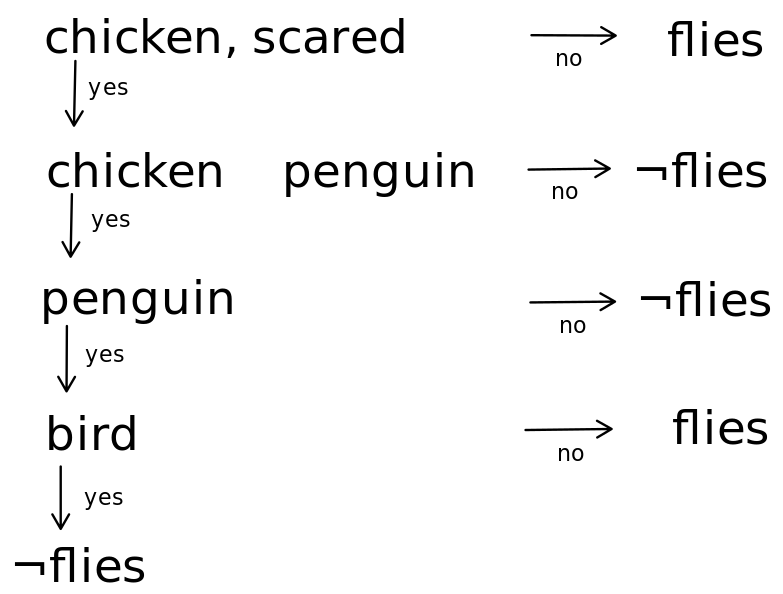
\includegraphics[width=0.4\textwidth]{images/decision-list.png}
        \caption{A fictitious decision list.}
        \label{fig:decision-list}
\end{figure}

A decision list is a special kind of decision tree, where all questions are arranged a single branch \cite[ch.~18.5.1]{russellArtificialIntelligenceModern2010}. It can be mined similarly to normal decision trees on attribute-value data, and has a similar efficiency. Similar to decision list miners are \textit{covering rule} algorithms. They create the same output as a decision list, but use the criterion of \textit{coverage} instead of the criterion of information gain. Covering rule algorithms are also used explicitly for mining defeasible rules, especially the \textit{HeRo} algorithm (see \autoref{sec:defeasible-rules}). 

A decision list is very similar to a list of rules with with a preference, and thus to a defeasible theory. % TODO there is some source that also says so, forgot where ...

\subsection{Learning probabilistic and causal models}

\begin{figure}[htb]
        \centering
        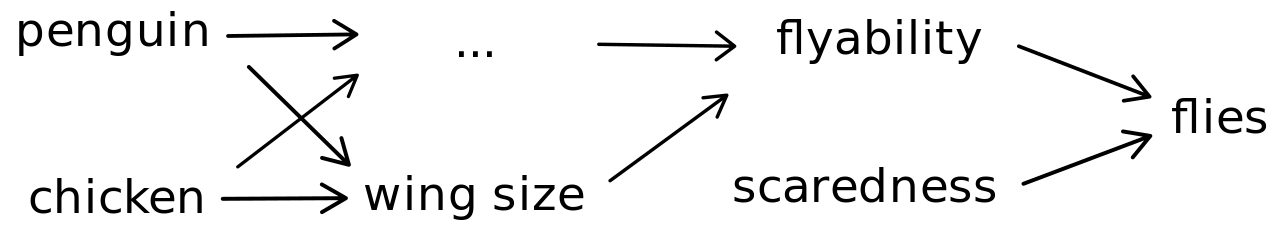
\includegraphics[width=0.7\textwidth]{images/causal-net.png}
        \caption{A fictitious causal probability network. To construct a proper causal network, variables that are hidden in the figures of the other approaches had to be introduced. The probability of each variable is a function (usually, a weighted sum or a logic table) of the probability of its parents; the functions are not further specified in this figure.}
        \label{fig:causal-network}
\end{figure}

Probability networks (Bayesian networks) are the most common tool for reasoning with uncertainty \citep[ch.~14.2]{russellArtificialIntelligenceModern2010}. They are used for attribute-value representations. In their general version, they are unsuitable for explainable artificial intelligence for three reasons, all of which have been addressed.

\begin{enumerate}
\item Probability networks contain numbers, and a lot of them. This is resolved by ignoring the numbers and instead just using positive and negative associations between variables. This is done in \textit{qualitative Bayesian networks}. Another approach is to replace probabilities with qualitative ranks, as is done in ranking theory. Ranking theory\footnote{\url{https://github.com/tjitze/RankPL}, \url{https://github.com/tjitze/ranked-programming}}\citep{spohnGeneralNonprobabilisticTheory1990,spohnLawsBeliefRanking2012} is a qualitative alternative to probability theory. It uses a preference relation on beliefs, and allows for basic reasoning. It has been applied to probability networks and especially to causal networks.
\item Probability networks may contain too many connections. A network will achieve the highest accuracy if it is fully connected. This makes reasoning hard both for the computer (addressable by sampling techniques) and, more importantly for us, for the human who tries to understand. This issue is resolved by training techniques for \textit{sparse Bayesian networks}. There, a regularization term penalizes the creation of connections, leading to networks with only a few connections. Reasonable networks with few connections are possible if the attributes of the training data describe a \textit{locally structured system} \cite[p.~516]{russellArtificialIntelligenceModern2010}.
\item Probability networks — as other rule-based techniques — are prone to causal misinterpretation. (That they are not causal is underlined by the fact that for the same data completely different valid networks can be constructed, depending on the order in which the nodes are processed during the construction of the network; see \citet[fig.~14.3]{russellArtificialIntelligenceModern2010}) This is resolved by using \textit{causal networks}, which actually allow for causal reasoning \citep{pearlCausalInferenceStatistics2016}. The construction of causal networks requires knowledge about the causal connections between the variables. This can be done in three ways: 
\begin{itemize}
    \item First, if the causal connections in the domain are fully understood, then humans can determine between which variables there are connections, and they can make sure that all confounding variables are included in the model.
    \item Second, if the causal theory of the domain is not fully understood, interventions can be undertaken and modelled using do-calculus to find out more about it. \citet{pearlCausalInferenceStatistics2016} emphasizes that such interventions are more flexible than randomized controlled trials.
    \item A third approach tries to learn causal connections from the observational training data alone; see, for example, \cite{wallaceCausalDiscoveryMML1996}.
\end{itemize}
\end{enumerate}

The links in causal networks can be regarded as causal rules. When we want to determine which action we want to take, these rules are the only kind of rules that can help us. All the other approaches that are presented here only take into consideration statistical associations, which cannot in general be used to reason about the consequences of interventions.

% \section{Data sets}

\section{Propositionalization}

As mentioned in \autoref{without}, we will try to transfer the approach from \citet{verheijProofProbabilities2017} to work on propositional data. This requires that continuous attributes be converted to boolean (or, propositional values). On a theoretical level, this idea is explored in \citet{deraedtLogicalRelationalLearning2008}. Here we present practical approaches for propositionalization. Propositionalization of multiple attributes at once is known as \textit{clustering}, and may also be relevant for our approach.

\subsection{Equal-Width Partitioning}

This is the simplest clustering approach considered. Here, the range of the variable is divided into $k$ bins, each of size $\frac{Max-Min}{k}$ (where $Max$ and $Min$ refer to the maximum and minimum value of the variable, respectively).

This approach is easy to implement and not computationally expensive. However, there are some notable flaws: This algorithm assumes that each cluster has the same diameter, and it is prone to outliers.

\subsection{Equal-Depth Partitioning}

Another simple algorithm is known as equal-depth partitioning. Here, the clusters are built in such a way that each of them hold the same number of instances.

This could prove to be problematic as not all clusters necessarily have this property.

\subsection{K-Means }

K-Means\citep{lloydLeastSquaresQuantization1982} is based on the idea of centroids, which are points in the centre of the cluster. Here, k centroids are initialized randomly, and the instances are assigned to the cluster whose centroid is closest. Then, the centroids are moved to the mean of the cluster, and the instances are assigned to their new cluster. This pattern is repeated until the algorithm converges.

One flaw of this algorithm is that it may be sensitive to outliers. To make it more robust to noise, the centroids can take on the median value. Alternatively, the instance closest to the average of the cluster can be referred to as the centroid of the cluster.

Another flaw of this algorithm is that it is highly dependant on the random initialization. Therefore, this algorithm must run multiple times to ensure the best clusters are found. (To evaluate the clusters, the 'silhouette score' explained later in this section can be used.)

Lastly, the algorithm is built on the assumption that every cluster has a similar diameter, which may not be true for some datasets.

\subsection{DBSCAN}

This algorithm considers clusters to be regions of high density. To find the clusters, the algorithm counts the number of instances within a distance defined by $\epsilon$, also called the instance's $\epsilon$-neighbourhood. If this number of neighbours of an instance surpasses a predefined threshold, the instance is considered to be a \textit{core instance}, an instance within a dense region. The neighbours of this core instance are considered to be in the same cluster, where some neighbours may also be core instances themselves. Therefore, a cluster consists of a multitude of core instances.


